\chapter{Object Segmentation Results Comparison}
\label{app:seg_results}

\begin{figure}[htb]
    \begin{tabular}{ccc}
    	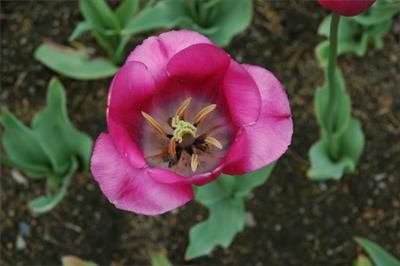
\includegraphics[width=0.3\textwidth]{interface/segmentation/tests/1.jpg}        &
    	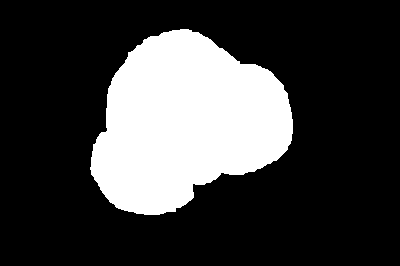
\includegraphics[width=0.3\textwidth]{interface/segmentation/tests/1.png}    & 						
    	
\includegraphics[width=0.3\textwidth]{interface/segmentation/tests/1_res.png}   \\
    	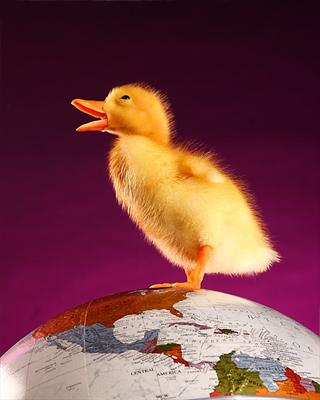
\includegraphics[width=0.3\textwidth]{interface/segmentation/tests/2.jpg}        &
    	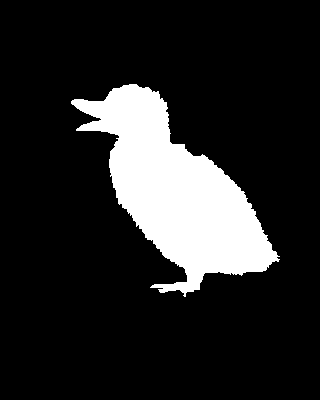
\includegraphics[width=0.3\textwidth]{interface/segmentation/tests/2.png}    & 						
    	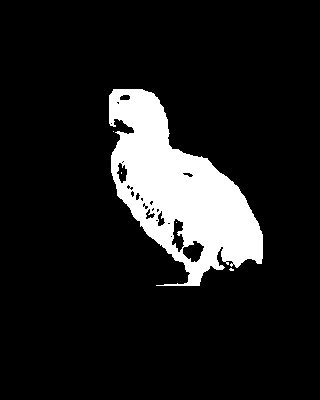
\includegraphics[width=0.3\textwidth]{interface/segmentation/tests/2_res.png}   \\
    	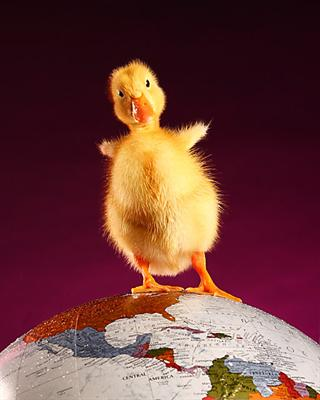
\includegraphics[width=0.3\textwidth]{interface/segmentation/tests/3.jpg}        &
    	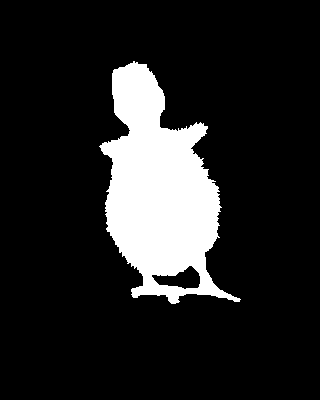
\includegraphics[width=0.3\textwidth]{interface/segmentation/tests/3.png}    & 						
    	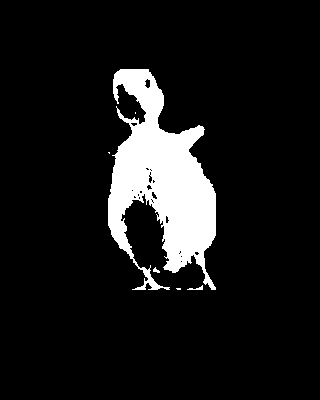
\includegraphics[width=0.3\textwidth]{interface/segmentation/tests/3_res.png}   \\
    	(a) & (b) & (c)
    \end{tabular}	
    \caption{Example of correct object segmentation of the implemented algorithm (c)  only using the pixels considered as foreground in comparison to the original algorithm (b) \cite{cheng2011global}.}
\end{figure}


\begin{figure}[htb]
    \begin{tabular}{ccc}
    	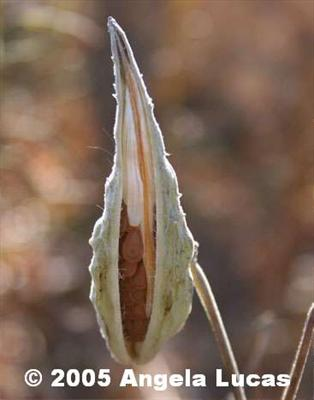
\includegraphics[width=0.3\textwidth]{interface/segmentation/tests/4.jpg}        &
    	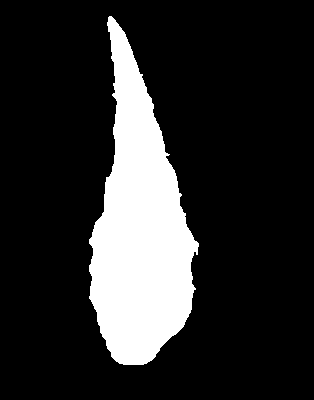
\includegraphics[width=0.3\textwidth]{interface/segmentation/tests/4.png}    & 						
    	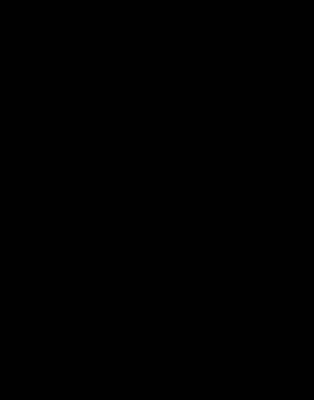
\includegraphics[width=0.3\textwidth]{interface/segmentation/tests/4_res.png}   \\
    	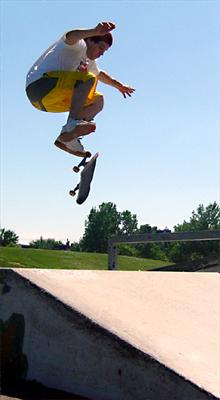
\includegraphics[width=0.3\textwidth]{interface/segmentation/tests/5.jpg}        &
    	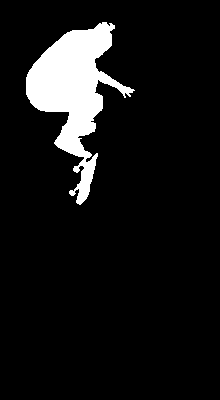
\includegraphics[width=0.3\textwidth]{interface/segmentation/tests/5.png}    & 						
    	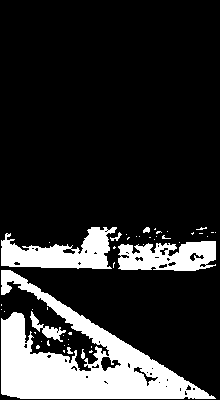
\includegraphics[width=0.3\textwidth]{interface/segmentation/tests/5_res.png}   \\
    	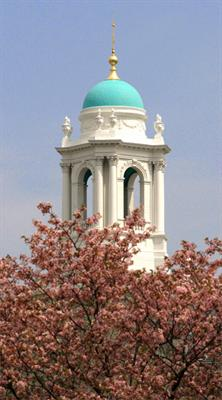
\includegraphics[width=0.3\textwidth]{interface/segmentation/tests/6.jpg}        &
    	
\includegraphics[width=0.3\textwidth]{interface/segmentation/tests/6.png}    & 						
    	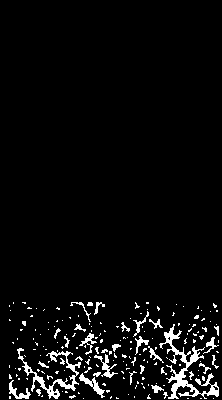
\includegraphics[width=0.3\textwidth]{interface/segmentation/tests/6_res.png}   \\
    	(a) & (b) & (c)
    \end{tabular}	
    \caption{Example of failed object segmentation of the implemented algorithm (c) only using the pixels considered as foreground in comparison to the original algorithm (b) \cite{cheng2011global}.}
\end{figure}

\begin{figure}[htb]
    \begin{tabular}{ccc}
    	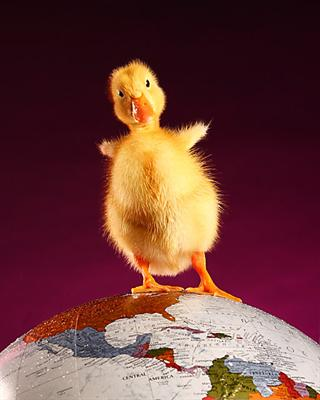
\includegraphics[width=0.3\textwidth]{interface/segmentation/tests/7.jpg}        &
    	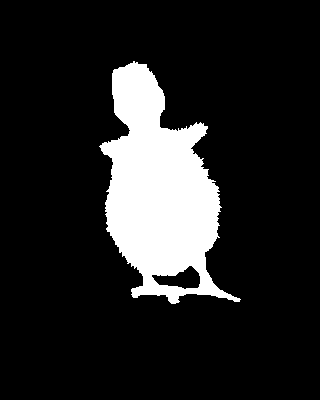
\includegraphics[width=0.3\textwidth]{interface/segmentation/tests/7.png}    & 						
    	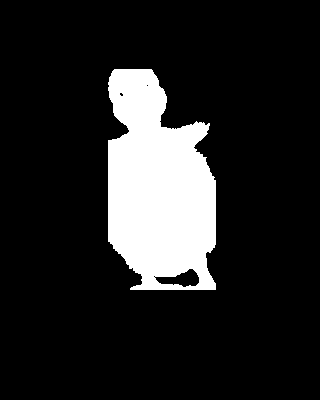
\includegraphics[width=0.3\textwidth]{interface/segmentation/tests/7_res.png}   \\
    	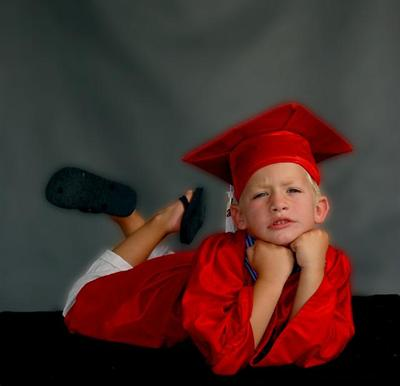
\includegraphics[width=0.3\textwidth]{interface/segmentation/tests/8.jpg}        &
    	
\includegraphics[width=0.3\textwidth]{interface/segmentation/tests/8.png}    & 						
    	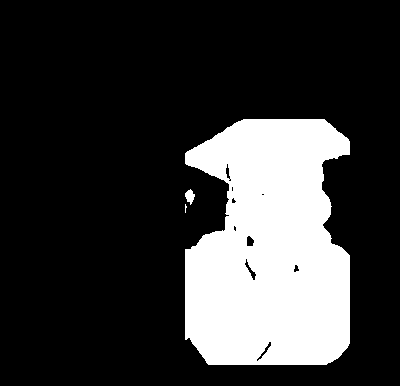
\includegraphics[width=0.3\textwidth]{interface/segmentation/tests/8_res.png}   \\
    	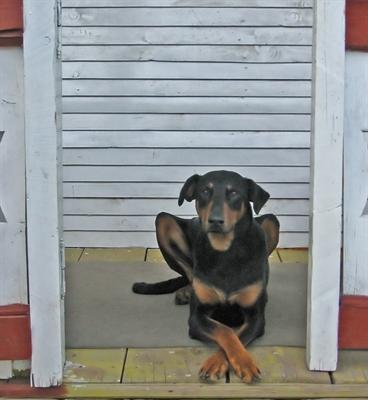
\includegraphics[width=0.3\textwidth]{interface/segmentation/tests/9.jpg}        &
    	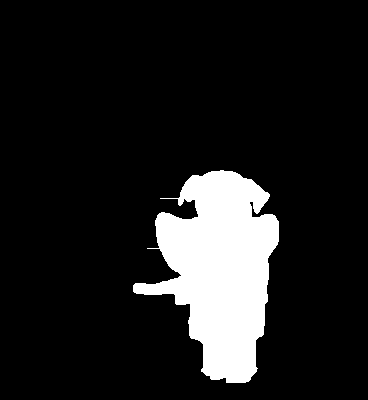
\includegraphics[width=0.3\textwidth]{interface/segmentation/tests/9.png}    & 						
    	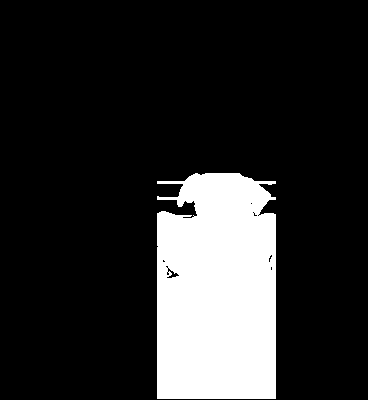
\includegraphics[width=0.3\textwidth]{interface/segmentation/tests/9_res.png}   \\
    	(a) & (b) & (c)
    \end{tabular}	
    \caption{Example of correct object segmentation of the implemented algorithm (c) using the pixels considered as foreground and background in comparison to the original algorithm (b) \cite{cheng2011global}.}
\end{figure}